%%this is /book/sciwms.tex
\section{\sciwms{}}
\label{sec:sciwms}
\subsection{Overview}
\Sciwms{} is an open-source implementation of the Open Geospatial
Consortium's (\ogc{}) Web Map Service (\wms{}) standard which
specifies an HTTP interface for generating rasterized visualizations
of geospatial data~\cite{wms14}. \sciwms{} is implemented in Python
using the Django~\cite{django} web framework and standard
cross-platform numerical software, NumPy~\cite{numpy11} and
Matplotlib~\cite{hunter07} for generating visual
content. Additionally, the open-source python implementation provides
a cross-platform \wms{} solution which can leverage the suite of tools
developed by the geospatial data analysis community, such as
pyugrid~\cite{pyugrid}, to maintain pace with the latest geospatial
software and standards developments including unstructured grid support
and \cfugrid{} Compliance~\cite{cfugrid}.



Vital to the efficiency of \sciwms{} is the abstraction of a dataset
into two entities: a topology, defined as a geo-referenced spatial
structure and numerical data attributes. \Sciwms{} creates a local
topology cache for efficiently computing spatial neighborhoods and
subsets with respect to topology structure. For storage efficiency,
attributes associated with the topology is not replicated locally but
referenced via OGC compliant web-services and a database of
topology-endpoint pairs is maintained as visualized in
figure~\ref{fig:sciwms_topology_endpoints}. Because geospatial \wms{}
requests are commonly restricted to a subset of the Earth's surface,
\sciwms{} uses the local topology to compute the subset of model data
needed to fulfill each request prior to accessing the external
data. Furthermore, by classifying topologies as either regular or
unstructured, efficient algorithms and data structures are exploited
to optimize the computation of relevant model data subsets.

%% \begin{figure}[ht!]
%%   \centering
%%   \includegraphics[width=0.7\columnwidth]{../figs/sciwms_overview_v2.pdf}
%%   \caption{Overview of the \sciwms{} deployment for the U.S. \ioos{}
%%     \comt{} project. \Sciwms{} updates its topology and endpoint
%%     database via a nightly service which queries CF-Compliant datasets
%%     cataloged by \ngdc{}. Model data is hosted on an external web server
%%     exposed by an \ncml{} facade as a single \netcdf{} data structure
%%     accessable to \sciwms{} via \opendap{}. \Sciwms{} responds to http
%%     clients interfacing through a custom built web portal.}
%%   \label{fig:overview1}
%% \end{figure}
%% \begin{figure}[ht!]
%%   \centering
%%   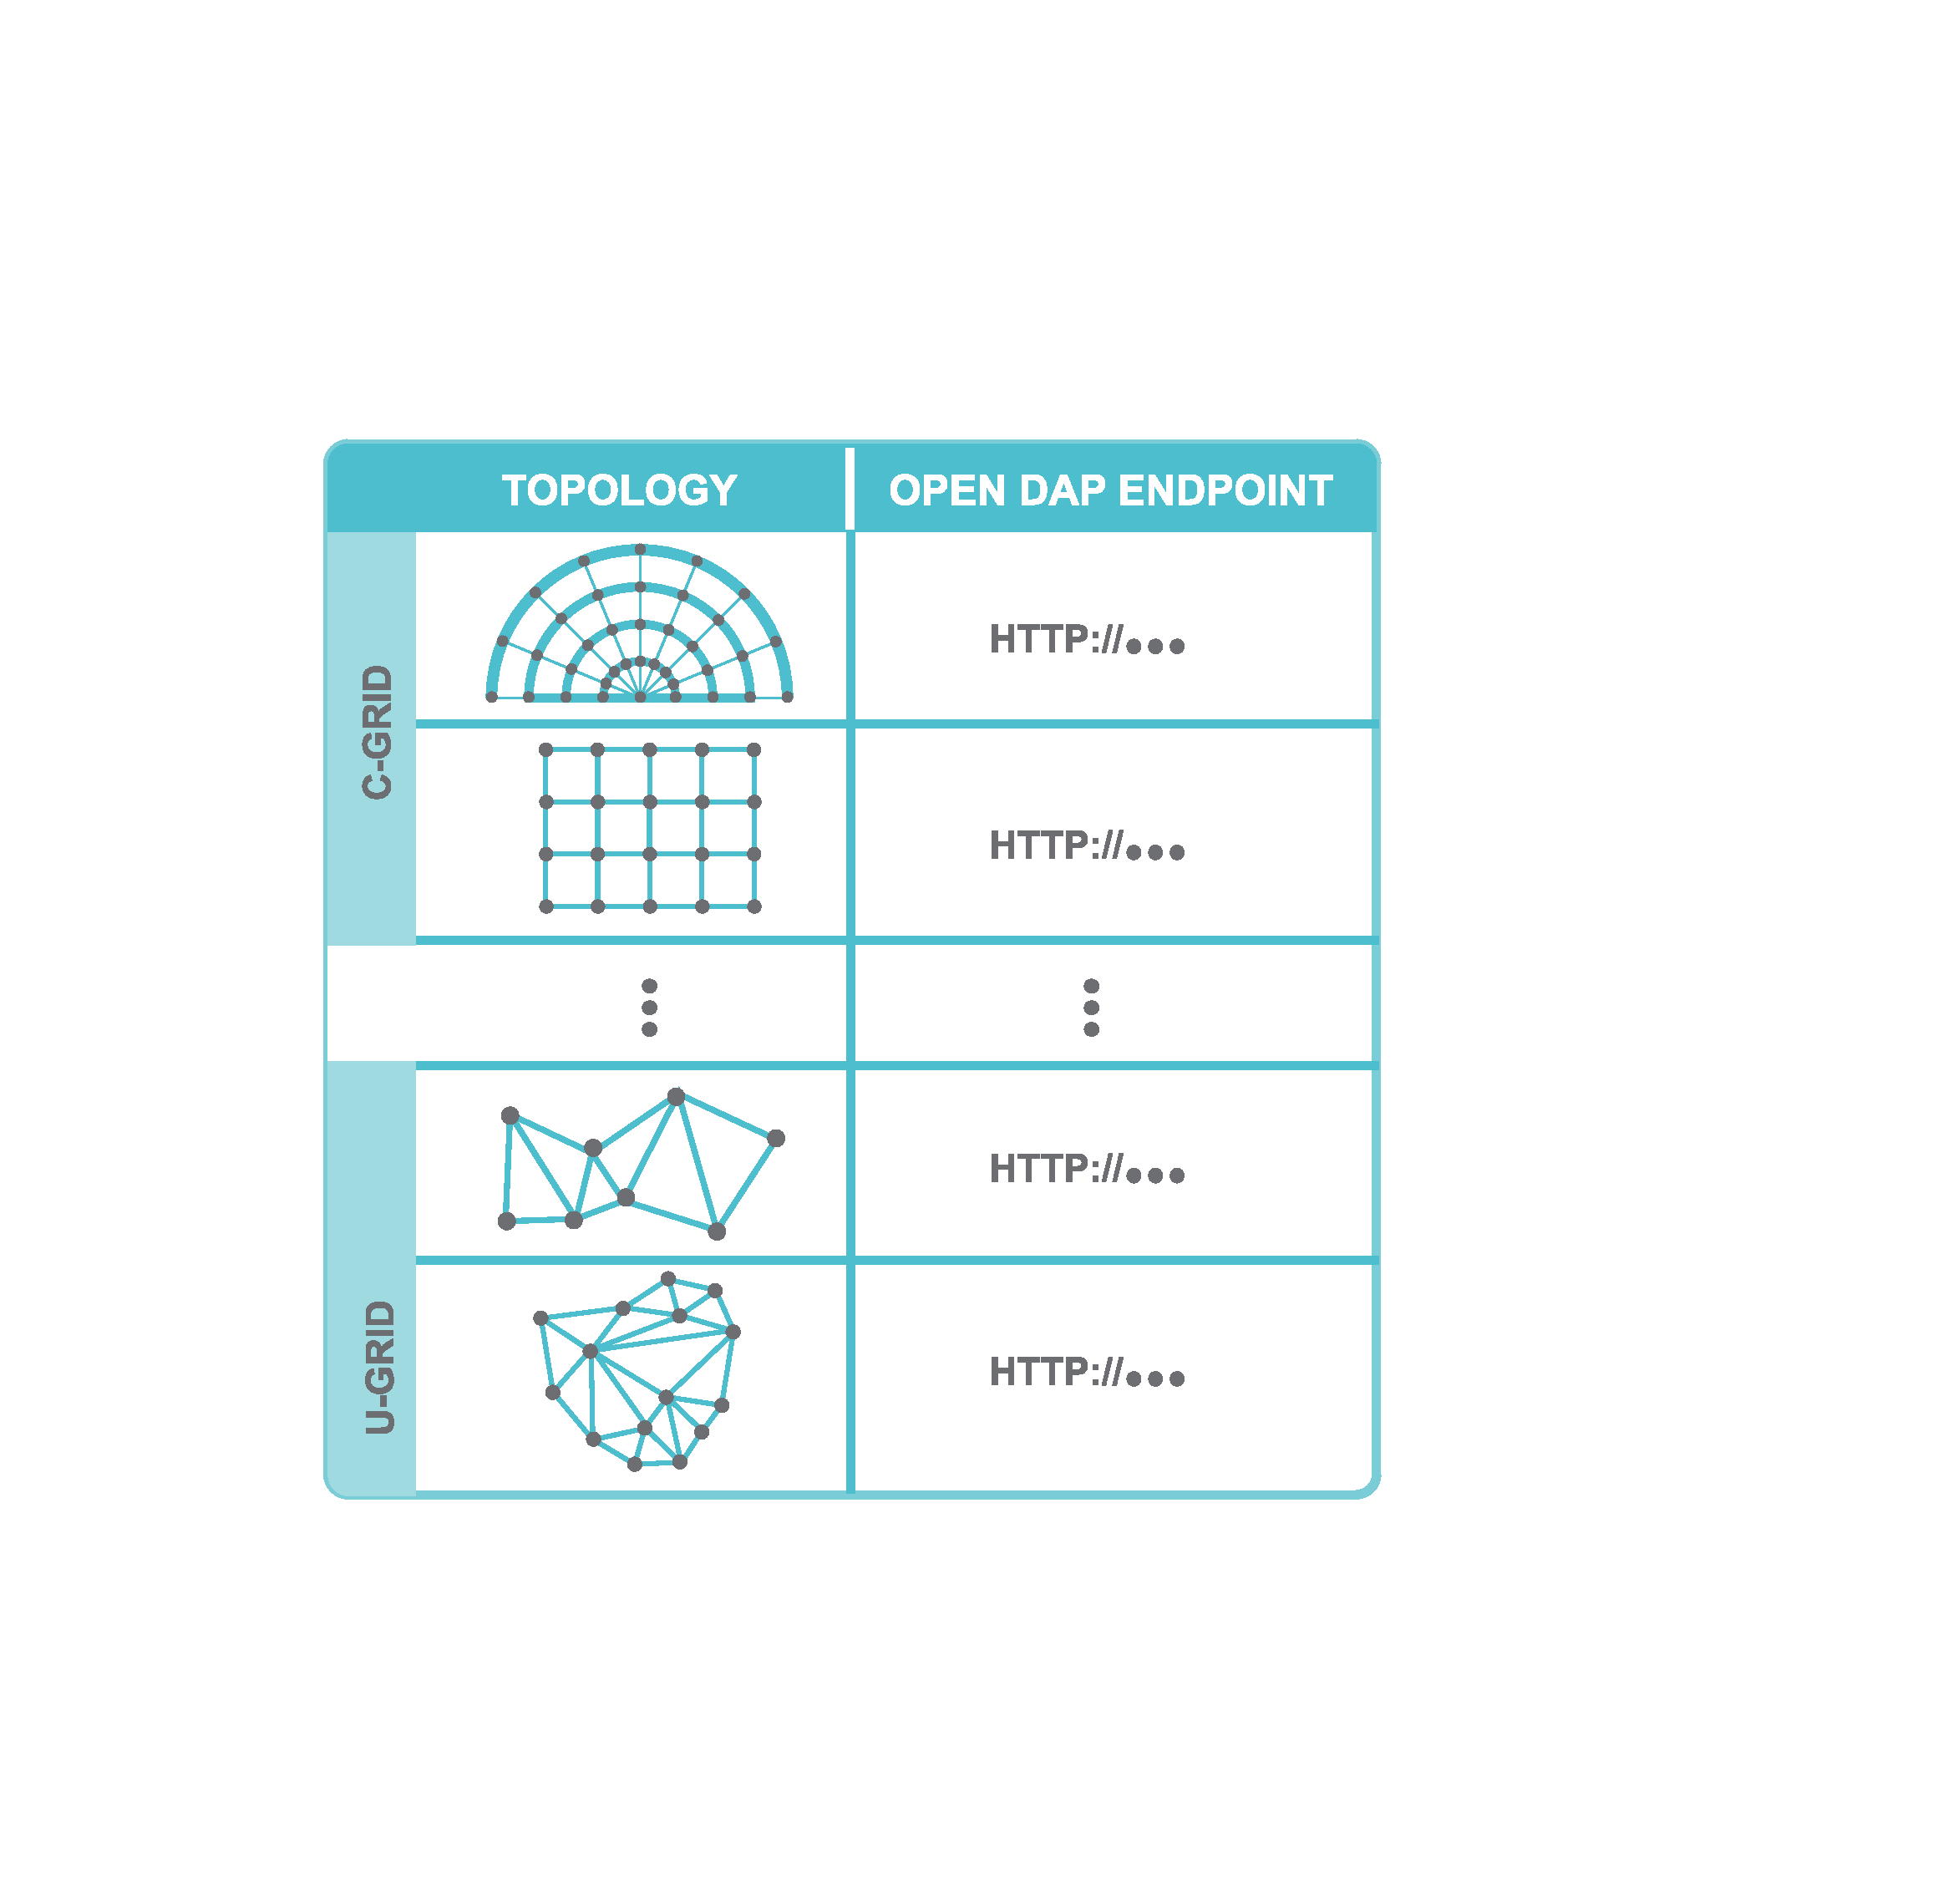
\includegraphics[width=0.6\columnwidth]{../figs/sciwms_book_db_topology_endpoints.pdf}
%%   \caption{\Sciwms{} topology and endpoint data store. Typologies are
%%     classified as \cgrid{} and \ugrid{} for efficient geospatial
%%     queries and remote model data access.}
%%   \label{fig:sciwms_topology_endpoints}
%% \end{figure}

\begin{figure}
  \centering
  \begin{subfigure}[b]{0.455\textwidth}
    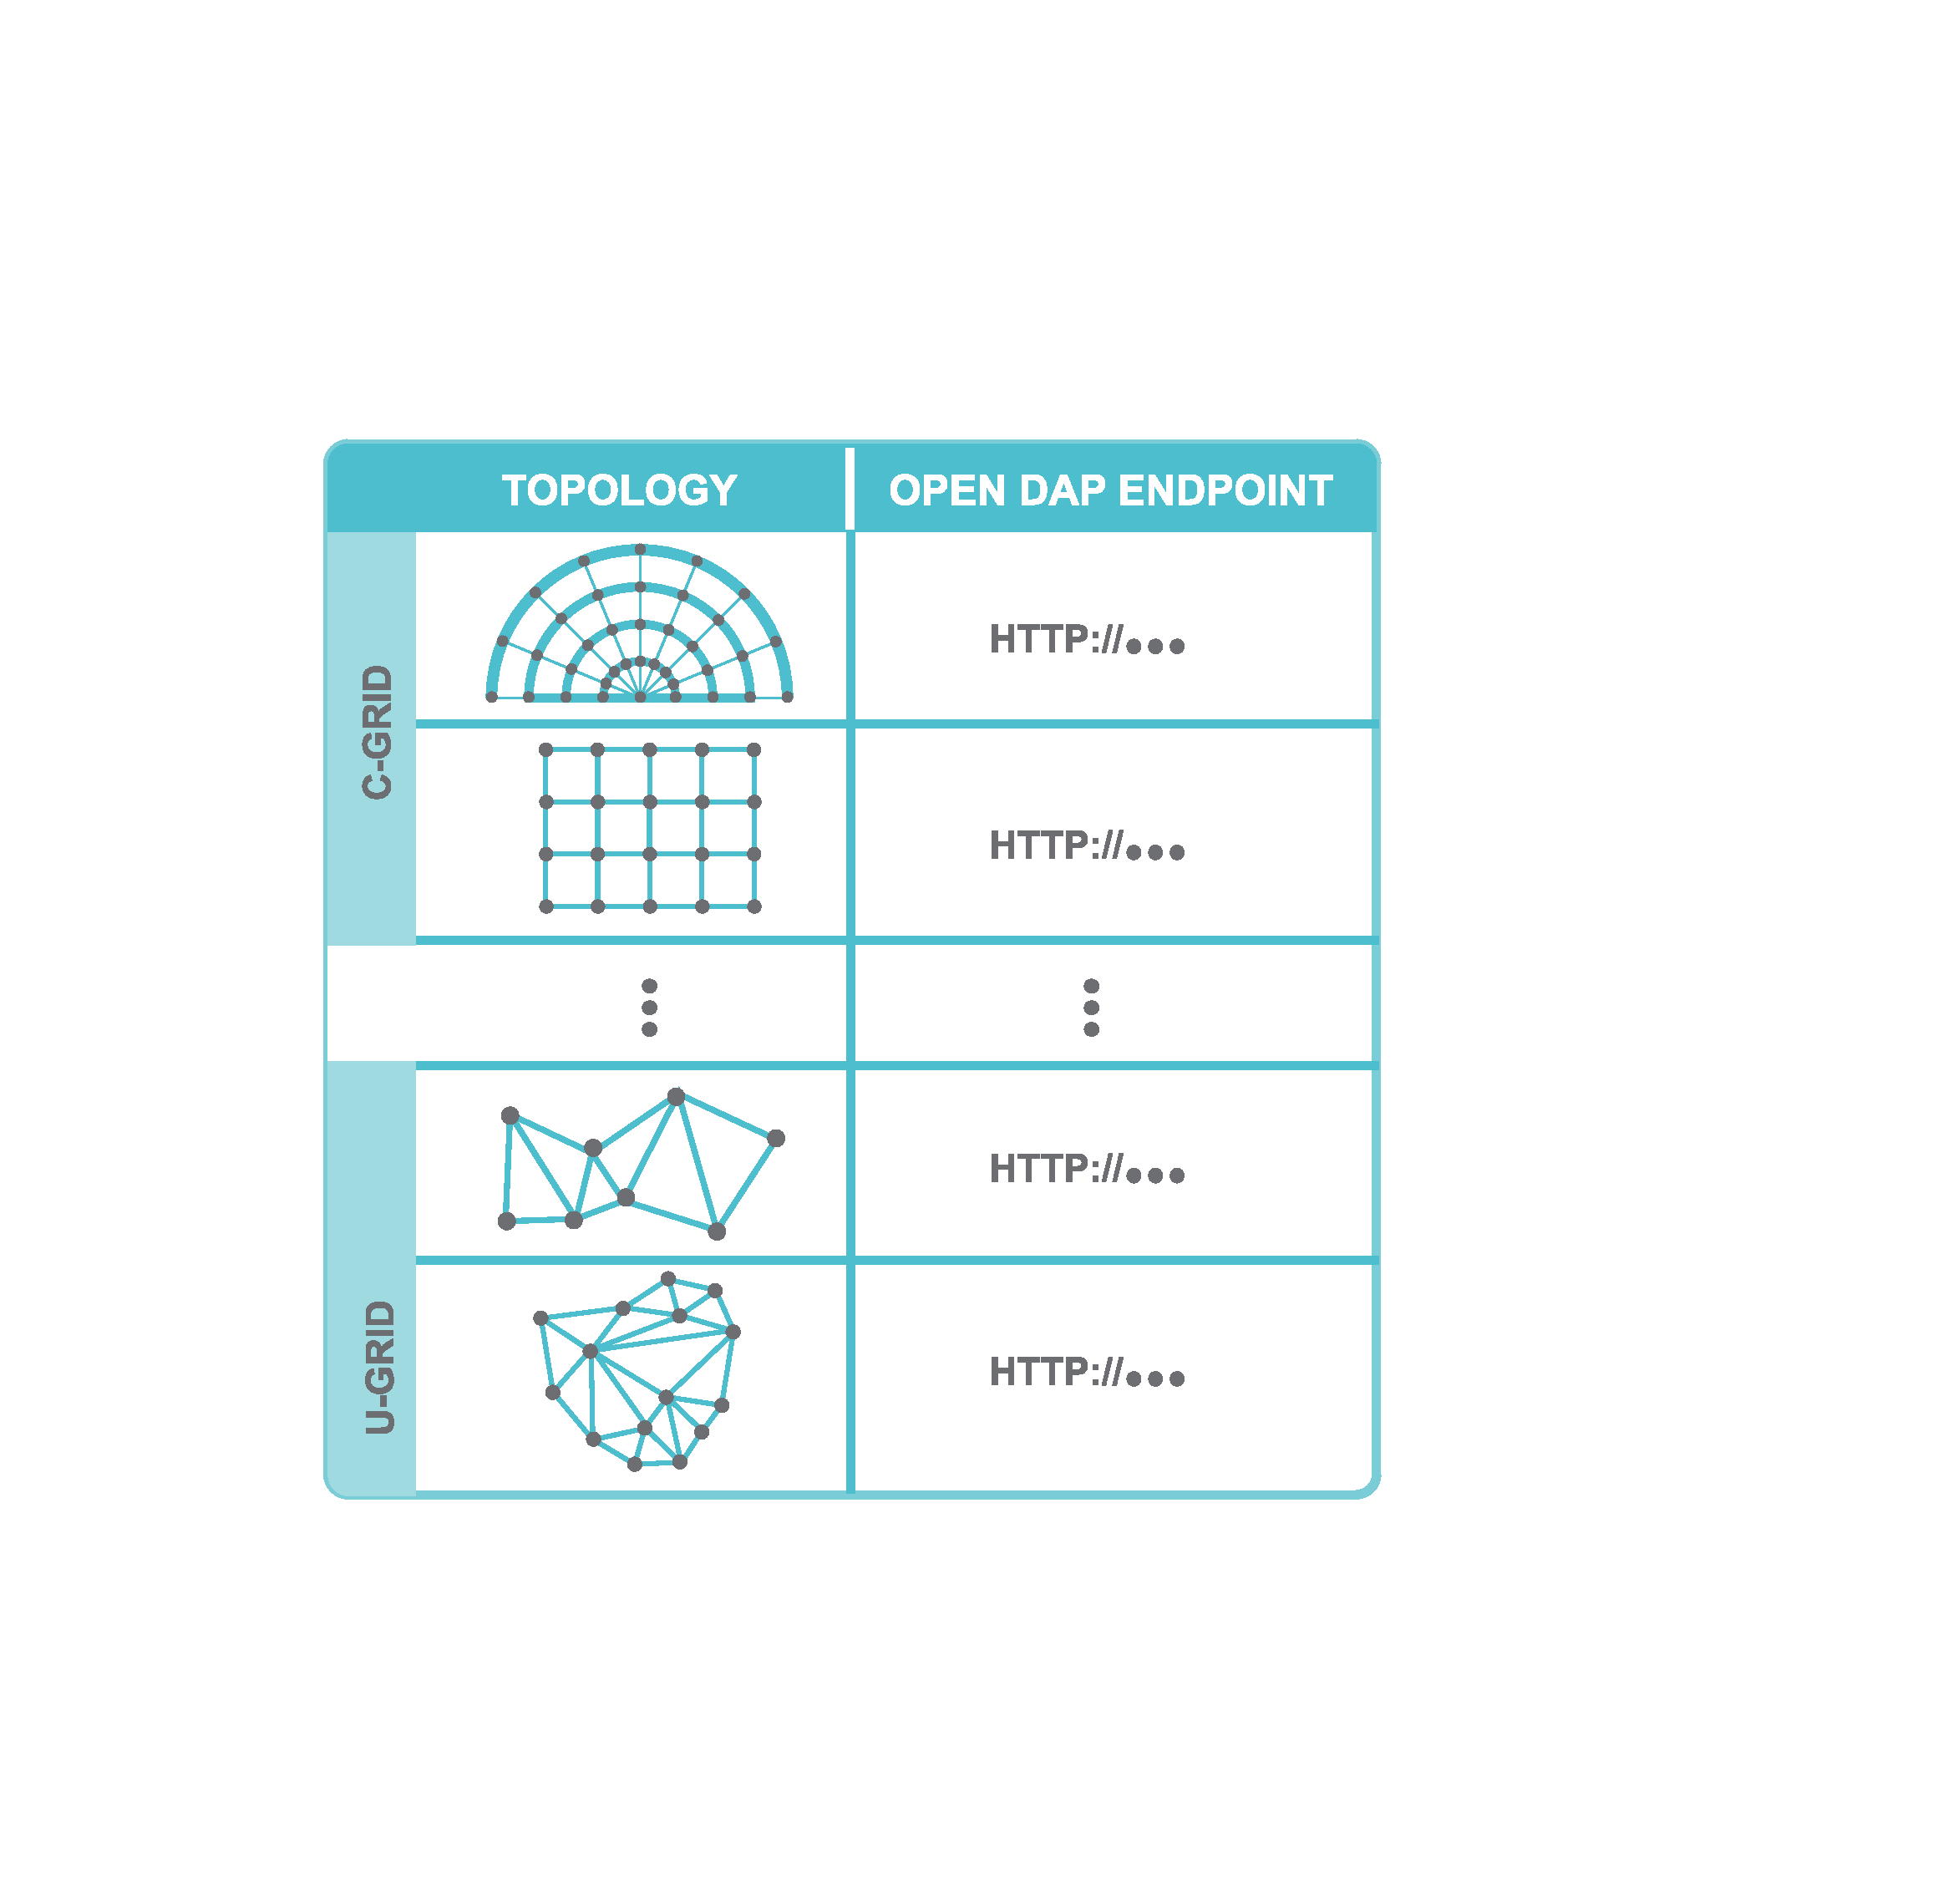
\includegraphics[width=\textwidth]{../figs/sciwms_book_db_topology_endpoints.pdf}
    \caption{\Sciwms{} topology and endpoint data store.}
    \label{fig:sciwms_topology_endpoints}
  \end{subfigure}
  \begin{subfigure}[b]{0.45\textwidth}
    \includegraphics[width=\textwidth]{../figs/sciwms_overview_v2.pdf}
    \caption{Overview of the \sciwms{} deployment for the U.S. \ioos{}
      \comt{} project.}
    \label{fig:overview1}
  \end{subfigure}
  \caption{\sciwms{} architecture.}
  \label{fig:architecture}
\end{figure}


